\documentclass{article}\usepackage[]{graphicx}\usepackage[]{color}
% maxwidth is the original width if it is less than linewidth
% otherwise use linewidth (to make sure the graphics do not exceed the margin)
\makeatletter
\def\maxwidth{ %
  \ifdim\Gin@nat@width>\linewidth
    \linewidth
  \else
    \Gin@nat@width
  \fi
}
\makeatother

\definecolor{fgcolor}{rgb}{0.345, 0.345, 0.345}
\newcommand{\hlnum}[1]{\textcolor[rgb]{0.686,0.059,0.569}{#1}}%
\newcommand{\hlstr}[1]{\textcolor[rgb]{0.192,0.494,0.8}{#1}}%
\newcommand{\hlcom}[1]{\textcolor[rgb]{0.678,0.584,0.686}{\textit{#1}}}%
\newcommand{\hlopt}[1]{\textcolor[rgb]{0,0,0}{#1}}%
\newcommand{\hlstd}[1]{\textcolor[rgb]{0.345,0.345,0.345}{#1}}%
\newcommand{\hlkwa}[1]{\textcolor[rgb]{0.161,0.373,0.58}{\textbf{#1}}}%
\newcommand{\hlkwb}[1]{\textcolor[rgb]{0.69,0.353,0.396}{#1}}%
\newcommand{\hlkwc}[1]{\textcolor[rgb]{0.333,0.667,0.333}{#1}}%
\newcommand{\hlkwd}[1]{\textcolor[rgb]{0.737,0.353,0.396}{\textbf{#1}}}%
\let\hlipl\hlkwb

\usepackage{framed}
\makeatletter
\newenvironment{kframe}{%
 \def\at@end@of@kframe{}%
 \ifinner\ifhmode%
  \def\at@end@of@kframe{\end{minipage}}%
  \begin{minipage}{\columnwidth}%
 \fi\fi%
 \def\FrameCommand##1{\hskip\@totalleftmargin \hskip-\fboxsep
 \colorbox{shadecolor}{##1}\hskip-\fboxsep
     % There is no \\@totalrightmargin, so:
     \hskip-\linewidth \hskip-\@totalleftmargin \hskip\columnwidth}%
 \MakeFramed {\advance\hsize-\width
   \@totalleftmargin\z@ \linewidth\hsize
   \@setminipage}}%
 {\par\unskip\endMakeFramed%
 \at@end@of@kframe}
\makeatother

\definecolor{shadecolor}{rgb}{.97, .97, .97}
\definecolor{messagecolor}{rgb}{0, 0, 0}
\definecolor{warningcolor}{rgb}{1, 0, 1}
\definecolor{errorcolor}{rgb}{1, 0, 0}
\newenvironment{knitrout}{}{} % an empty environment to be redefined in TeX

\usepackage{alltt}
\usepackage{amsmath} %This allows me to use the align functionality.
                     %If you find yourself trying to replicate
                     %something you found online, ensure you're
                     %loading the necessary packages!
\usepackage{amsfonts}%Math font
\usepackage{graphicx}%For including graphics
\usepackage{hyperref}%For Hyperlinks
\hypersetup{colorlinks = true,citecolor=black}
\usepackage{natbib}        %For the bibliography
\bibliographystyle{apalike}%For the bibliography
\usepackage[margin=1.0in]{geometry}
\usepackage{float}
\IfFileExists{upquote.sty}{\usepackage{upquote}}{}
\begin{document}
\noindent \textbf{MA 354: Data Analysis -- Fall 2021 -- Due 10/8 at 5p}\\%\\ gives you a new line
\noindent \textbf{Homework 2:}\vspace{1em}\\
\emph{Complete the following opportunities to use what we've talked about in class. These questions will be graded for correctness, communication and succinctness. Ensure you show your work and explain your logic in a legible and refined submission.}\\\vspace{1em}
%Comments -- anything after % is not put into the PDF

The starting jobs will be applied in alphabetical order (last name) for question two.
\begin{enumerate}
  \item \textbf{Solver:} provide a solution, if possible, and reasoning for the solution. \textbf{Due to group 10/5 or earlier.}
  \item \textbf{Code Checker:} provides a first check of the solver's worked solutions and ensures they are correct with a solid interpretation. 
  \item \textbf{Checker} checks the solution for completeness, proposes and implements changes if agreed upon by the group. Provides a short paragraph summarizing the discussion of proposals and their reason for acceptance or non-acceptance.
  \item \textbf{Double Checker} checks the solution for completeness, communication and polish. The Double Checker ensures that the solution is correct and highly polished for submission.
\end{enumerate}

\noindent For subsequent questions student roles will move down one position. The rolls change as follows.
\begin{enumerate}
  \item \textbf{Solver} $\Longrightarrow$ \textbf{Code Checker}
  \item \textbf{Code Checker} $\Longrightarrow$ \textbf{Checker}
  \item \textbf{Checker} $\Longrightarrow$ \textbf{Double Checker}
  \item \textbf{Double Checker} $\Longrightarrow$ \textbf{Solver}
\end{enumerate}
While students have assigned jobs for each question I encourage students to help 
each other complete the homework in collaboration.
\newpage
\begin{enumerate}
%%%%%%%%%%%%%%%%%%%%%%%%%%%%%%%%%%%%%%%%%%%%%%%%%%%%%%%%%%%%%%%%%%%%%%%%%%%%%%%%%%%%%%%%%%%
%%%%%%%%%%%%%%%%%%%%%%%%%%%%%%%%%%%%%%%%%%%%%%%%%%%%%%%%%%%%%%%%%%%%%%%%%%%%%%%%%%%%%%%%%%%
%%%%%%%%%  Question 1
%%%%%%%%%%%%%%%%%%%%%%%%%%%%%%%%%%%%%%%%%%%%%%%%%%%%%%%%%%%%%%%%%%%%%%%%%%%%%%%%%%%%%%%%%%%
%%%%%%%%%%%%%%%%%%%%%%%%%%%%%%%%%%%%%%%%%%%%%%%%%%%%%%%%%%%%%%%%%%%%%%%%%%%%%%%%%%%%%%%%%%%
  \item\label{Q1} Select a continuous distribution (Not the uniform or exponential). 
  It does not have to be one that we cover in the notes! To explore the PDF of your 
  distribution, specify two sets of parameter(s) for your distribution.
  \begin{enumerate}
  %%%%%%%%%%%%%%%%%%%%%%%%%%%%%%%%%%%%%%%%%%%%%%%%%%%%%%%%%%%%%%%%%%%%%%%%%%%%%%%%%%%%%%%%%%%
  %%%%%%%%%  Part (a)
  %%%%%%%%%%%%%%%%%%%%%%%%%%%%%%%%%%%%%%%%%%%%%%%%%%%%%%%%%%%%%%%%%%%%%%%%%%%%%%%%%%%%%%%%%%%
  \item \textbf{History} Discuss what types of random variables are modeled with 
  your distribution. Be sure to include a discussion about the support and ensure 
  to provide the density function, and CDF. This requires some internet research 
  -- what's the history of the distribution, why was it created and named? What 
  are some exciting applications of this distribution?
  
  Cite all of your sources in LaTeX by adding a BibTeX citation to the .bib file. 
  To help, I've cited R \citep{R21} in parentheses here. \cite{R21} provides helpful 
  tools for the rest of the questions below. BibTeX citations are available through 
  Google Scholar by clicking the cite button below the article of  interest and 
  selecting the BibTeX option.
  %%%%%%%%%%%%%%%%%%%%%%%%%%%%%%%%%%%%%%%%%%%%%%%%%%%%%%%%%%%%%%%%%%%%%%%%%%%%%%%%%%%%%%%%%%%
  %%%%%%%%%  Part (b)
  %%%%%%%%%%%%%%%%%%%%%%%%%%%%%%%%%%%%%%%%%%%%%%%%%%%%%%%%%%%%%%%%%%%%%%%%%%%%%%%%%%%%%%%%%%%
	\item Show that you have a valid PDF. You will find the \texttt{integrate()} 
	function in \texttt{R} helpful.\\
	\textbf{Solution:}\\
	Here's the equation of PDF for normal distribution!
	\begin{equation*}
	f_{X}({x|\mu,\sigma})=\frac{1}{\sigma\sqrt{2\pi}}\exp^\frac{-(x-\mu)^2}{2\sigma^2} \tag{\textbf{PDF}}
	\end{equation*}
	Now, let's prove that it's valid!\\
	Since normal (or gaussian — whatever you prefer!) distribution is a continous probability distribution, it implies that the area under the curve is equal to 1 (or 100\%!). This statement takes its roots from the second Kolmogorov axiom that states that the entirety of sample space is equal to one.\\
	Therefore, let's use CDF to prove that our PDF formula is going to return one! Since the support for normal distribution contain all rational numbers, our integral is going to be from negative infinity to positive infinity. 
	\begin{equation*}
	F_{X}({x|\mu,\sigma})=\int_{-\infty}^{\infty}\frac{1}{\sigma\sqrt{2\pi}}\exp^\frac{-(x-\mu)^2}{2\sigma^2} \tag{\textbf{CDF}}
	\end{equation*}
	I am going to use \texttt{integrate()} function in order to compute this equation.
\begin{knitrout}
\definecolor{shadecolor}{rgb}{0.969, 0.969, 0.969}\color{fgcolor}\begin{kframe}
\begin{alltt}
\hlstd{mean}\hlkwb{<-}\hlnum{1} \hlcom{#mu}
\hlstd{sd}\hlkwb{<-}\hlnum{3} \hlcom{#sigma}
\hlstd{func} \hlkwb{<-} \hlkwa{function}\hlstd{(}\hlkwc{x}\hlstd{)\{}
  \hlstd{(}\hlnum{1}\hlopt{/}\hlstd{(sd}\hlopt{*}\hlkwd{sqrt}\hlstd{(}\hlnum{2}\hlopt{*}\hlstd{pi)))}\hlopt{*}\hlkwd{exp}\hlstd{((}\hlopt{-}\hlstd{(x}\hlopt{-}\hlstd{mean)}\hlopt{^}\hlnum{2}\hlstd{)}\hlopt{/}\hlstd{(}\hlnum{2}\hlopt{*}\hlstd{sd}\hlopt{^}\hlnum{2}\hlstd{))}
\hlstd{\}}
\hlkwd{integrate}\hlstd{(func,} \hlopt{-}\hlnum{Inf}\hlstd{,} \hlnum{Inf}\hlstd{)}
\end{alltt}
\begin{verbatim}
## 1 with absolute error < 2.1e-07
\end{verbatim}
\end{kframe}
\end{knitrout}
	
	%%%%%%%%%%%%%%%%%%%%%%%%%%%%%%%%%%%%%%%%%%%%%%%%%%%%%%%%%%%%%%%%%%%%%%%%%%%%%%%%%%%%%%%%%%%
  %%%%%%%%%  Part (c)
  %%%%%%%%%%%%%%%%%%%%%%%%%%%%%%%%%%%%%%%%%%%%%%%%%%%%%%%%%%%%%%%%%%%%%%%%%%%%%%%%%%%%%%%%%%%
	\item Find the median for your two sets of parameter(s). Conduct some research 
	to find the median based on our PDF to confirm that your numerical approach is 
	correct. \\
	\textbf{Solution:}\\
	As we have established in part \texttt{(a)} of this problem, one of the key features of the normal distribution is the fact that it's symmetrical. Let's set out to prove it through the direct proof!\\
		Let \texttt{m} be median!
		\begin{equation*}
	P(X\le m)=P(X\ge m)=\frac{1}{2}
	\tag{\textbf{Definition of the median}}
	\end{equation*}
	Let normal distribution be symmetric. If it's symmetric, then the statement $\mu=m$ holds true.\\
	Therefore, the following equation should also hold true:
	\begin{equation*}
\int_{-\infty}^{\mu}\frac{1}{\sigma\sqrt{2\pi}}\exp^\frac{-(x-\mu)^2}{2\sigma^2}=
\int_{\mu}^{\infty}\frac{1}{\sigma\sqrt{2\pi}}\exp^\frac{-(x-\mu)^2}{2\sigma^2}=
\frac{1}{2}
\tag{\textbf{Assumption}}
	\end{equation*}
	
	Let's check it through R!
\begin{knitrout}
\definecolor{shadecolor}{rgb}{0.969, 0.969, 0.969}\color{fgcolor}\begin{kframe}
\begin{alltt}
        \hlstd{mean}\hlkwb{<-}\hlnum{1} \hlcom{#mu}
        \hlstd{sd}\hlkwb{<-}\hlnum{3} \hlcom{#sigma}
        \hlstd{func} \hlkwb{<-} \hlkwa{function}\hlstd{(}\hlkwc{x}\hlstd{)\{}
          \hlstd{(}\hlnum{1}\hlopt{/}\hlstd{(sd}\hlopt{*}\hlkwd{sqrt}\hlstd{(}\hlnum{2}\hlopt{*}\hlstd{pi)))}\hlopt{*}\hlkwd{exp}\hlstd{((}\hlopt{-}\hlstd{(x}\hlopt{-}\hlstd{mean)}\hlopt{^}\hlnum{2}\hlstd{)}\hlopt{/}\hlstd{(}\hlnum{2}\hlopt{*}\hlstd{sd}\hlopt{^}\hlnum{2}\hlstd{))}
        \hlstd{\}}
        \hlstd{firstPart} \hlkwb{<-} \hlkwd{integrate}\hlstd{(func,} \hlopt{-}\hlnum{Inf}\hlstd{, mean)}
        \hlstd{secondPart} \hlkwb{<-} \hlkwd{integrate}\hlstd{(func, mean,} \hlnum{Inf}\hlstd{)}

        \hlstd{(firstPart}\hlopt{$}\hlstd{value)}
\end{alltt}
\begin{verbatim}
## [1] 0.5
\end{verbatim}
\begin{alltt}
        \hlstd{(firstPart}\hlopt{$}\hlstd{value}\hlopt{==}\hlstd{secondPart}\hlopt{$}\hlstd{value)}
\end{alltt}
\begin{verbatim}
## [1] TRUE
\end{verbatim}
\end{kframe}
\end{knitrout}

It would appear that $\mu=m!$ Therefore, mean is equal to median within the normal distribution. Therefore, since $\mu_{1}=1$ and $\mu_{2}=-2$, the medians are 1 and -2 respectively!
	%%%%%%%%%%%%%%%%%%%%%%%%%%%%%%%%%%%%%%%%%%%%%%%%%%%%%%%%%%%%%%%%%%%%%%%%%%%%%%%%%%%%%%%%%%%
  %%%%%%%%%  Part (d)
  %%%%%%%%%%%%%%%%%%%%%%%%%%%%%%%%%%%%%%%%%%%%%%%%%%%%%%%%%%%%%%%%%%%%%%%%%%%%%%%%%%%%%%%%%%%
	\item \label{q1PDF} Graph the PDF for several values of the parameter(s) 
	including the two sets you specified. What does changing the parameter(s) do 
	to the shape of the PDF?\\
	\textbf{Solution:}\\
	Let's take various values and plot different PDFs! I am going to use QUOTE ggplot2 library for it!
\begin{figure}[H]
\begin{center}
\begin{knitrout}
\definecolor{shadecolor}{rgb}{0.969, 0.969, 0.969}\color{fgcolor}\begin{kframe}
\begin{alltt}
\hlkwd{library}\hlstd{(ggplot2)}
\hlstd{plot.df} \hlkwb{<-} \hlkwd{data.frame}\hlstd{(}
  \hlkwc{x}\hlstd{=}\hlkwd{seq}\hlstd{(}\hlopt{-}\hlnum{10}\hlstd{,} \hlnum{10}\hlstd{,} \hlnum{0.001}\hlstd{),}
  \hlkwc{f1}\hlstd{=}\hlkwd{dnorm}\hlstd{(}\hlkwc{x}\hlstd{=}\hlkwd{seq}\hlstd{(}\hlopt{-}\hlnum{10}\hlstd{,} \hlnum{10}\hlstd{,} \hlnum{0.001}\hlstd{),} \hlkwc{mean}\hlstd{=}\hlnum{1}\hlstd{,} \hlkwc{sd}\hlstd{=}\hlnum{1}\hlstd{),}
  \hlkwc{f2}\hlstd{=}\hlkwd{dnorm}\hlstd{(}\hlkwc{x}\hlstd{=}\hlkwd{seq}\hlstd{(}\hlopt{-}\hlnum{10}\hlstd{,} \hlnum{10}\hlstd{,} \hlnum{0.001}\hlstd{),} \hlkwc{mean}\hlstd{=}\hlopt{-}\hlnum{2}\hlstd{,} \hlkwc{sd}\hlstd{=}\hlnum{4}\hlstd{),}
  \hlkwc{f3}\hlstd{=}\hlkwd{dnorm}\hlstd{(}\hlkwc{x}\hlstd{=}\hlkwd{seq}\hlstd{(}\hlopt{-}\hlnum{10}\hlstd{,} \hlnum{10}\hlstd{,} \hlnum{0.001}\hlstd{),} \hlkwc{mean}\hlstd{=}\hlnum{0}\hlstd{,} \hlkwc{sd}\hlstd{=}\hlnum{5}\hlstd{),}
  \hlkwc{f4}\hlstd{=}\hlkwd{dnorm}\hlstd{(}\hlkwc{x}\hlstd{=}\hlkwd{seq}\hlstd{(}\hlopt{-}\hlnum{10}\hlstd{,} \hlnum{10}\hlstd{,} \hlnum{0.001}\hlstd{),} \hlkwc{mean}\hlstd{=}\hlnum{3}\hlstd{,} \hlkwc{sd}\hlstd{=}\hlnum{10}\hlstd{)}
\hlstd{)}

\hlkwd{ggplot}\hlstd{(plot.df,} \hlkwd{aes}\hlstd{(}\hlkwc{x}\hlstd{=x))}\hlopt{+}
  \hlkwd{geom_line}\hlstd{(}\hlkwd{aes}\hlstd{(}\hlkwc{y}\hlstd{=f1,} \hlkwc{color}\hlstd{=}\hlstr{"m=1, sd=1"}\hlstd{))}\hlopt{+}
  \hlkwd{geom_line}\hlstd{(}\hlkwd{aes}\hlstd{(}\hlkwc{y}\hlstd{=f2,} \hlkwc{color}\hlstd{=}\hlstr{"m=-2, sd=4"}\hlstd{))}\hlopt{+}
  \hlkwd{geom_line}\hlstd{(}\hlkwd{aes}\hlstd{(}\hlkwc{y}\hlstd{=f3,} \hlkwc{color}\hlstd{=}\hlstr{"m=0, sd=5"}\hlstd{))}\hlopt{+}
  \hlkwd{geom_line}\hlstd{(}\hlkwd{aes}\hlstd{(}\hlkwc{y}\hlstd{=f4,} \hlkwc{color}\hlstd{=}\hlstr{"m=3, sd=10"}\hlstd{))}
\end{alltt}
\end{kframe}
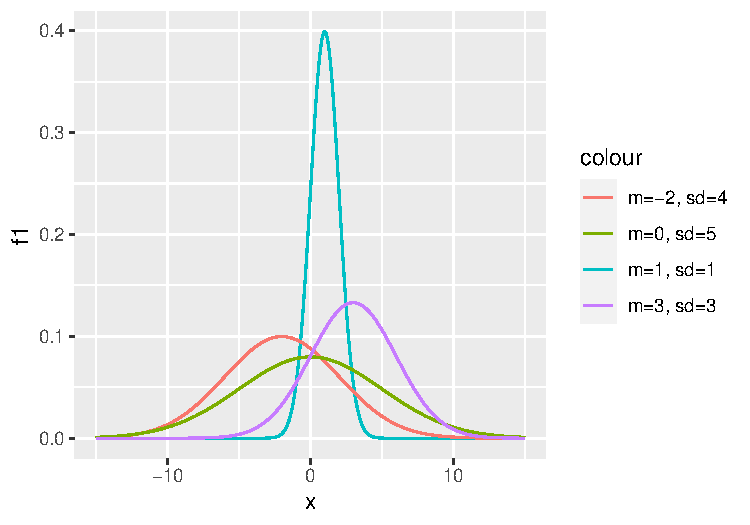
\includegraphics[width=\maxwidth]{figure/unnamed-chunk-3-1} 
\end{knitrout}
\caption{Gaussian PDF with various sets of parameters}
\label{plot1} %we can now reference plot1
\end{center}
\end{figure}
	%%%%%%%%%%%%%%%%%%%%%%%%%%%%%%%%%%%%%%%%%%%%%%%%%%%%%%%%%%%%%%%%%%%%%%%%%%%%%%%%%%%%%%%%%%%
  %%%%%%%%%  Part (e)
  %%%%%%%%%%%%%%%%%%%%%%%%%%%%%%%%%%%%%%%%%%%%%%%%%%%%%%%%%%%%%%%%%%%%%%%%%%%%%%%%%%%%%%%%%%%
	 \item Graph the CDF for the same values of the parameter(s) as you did in 
	 Question \ref{q1PDF}. What does changing the parameter(s) do to the shape of 
	 the CDF? Comment on the aspects of the CDFs that show that the CDF is valid.\\
	 \textbf{Solution:}\\
\begin{figure}[H]
\begin{center}
\begin{knitrout}
\definecolor{shadecolor}{rgb}{0.969, 0.969, 0.969}\color{fgcolor}\begin{kframe}
\begin{alltt}
\hlkwd{library}\hlstd{(ggplot2)}
\hlstd{plot.df} \hlkwb{<-} \hlkwd{data.frame}\hlstd{(}
  \hlkwc{x}\hlstd{=}\hlkwd{seq}\hlstd{(}\hlopt{-}\hlnum{10}\hlstd{,} \hlnum{10}\hlstd{,} \hlnum{0.001}\hlstd{),}
  \hlkwc{f1}\hlstd{=}\hlkwd{pnorm}\hlstd{(}\hlkwc{q}\hlstd{=}\hlkwd{seq}\hlstd{(}\hlopt{-}\hlnum{10}\hlstd{,} \hlnum{10}\hlstd{,} \hlnum{0.001}\hlstd{),} \hlkwc{mean}\hlstd{=}\hlnum{1}\hlstd{,} \hlkwc{sd}\hlstd{=}\hlnum{1}\hlstd{),}
  \hlkwc{f2}\hlstd{=}\hlkwd{pnorm}\hlstd{(}\hlkwc{q}\hlstd{=}\hlkwd{seq}\hlstd{(}\hlopt{-}\hlnum{10}\hlstd{,} \hlnum{10}\hlstd{,} \hlnum{0.001}\hlstd{),} \hlkwc{mean}\hlstd{=}\hlopt{-}\hlnum{2}\hlstd{,} \hlkwc{sd}\hlstd{=}\hlnum{4}\hlstd{),}
  \hlkwc{f3}\hlstd{=}\hlkwd{pnorm}\hlstd{(}\hlkwc{q}\hlstd{=}\hlkwd{seq}\hlstd{(}\hlopt{-}\hlnum{10}\hlstd{,} \hlnum{10}\hlstd{,} \hlnum{0.001}\hlstd{),} \hlkwc{mean}\hlstd{=}\hlnum{0}\hlstd{,} \hlkwc{sd}\hlstd{=}\hlnum{5}\hlstd{),}
  \hlkwc{f4}\hlstd{=}\hlkwd{pnorm}\hlstd{(}\hlkwc{q}\hlstd{=}\hlkwd{seq}\hlstd{(}\hlopt{-}\hlnum{10}\hlstd{,} \hlnum{10}\hlstd{,} \hlnum{0.001}\hlstd{),} \hlkwc{mean}\hlstd{=}\hlnum{3}\hlstd{,} \hlkwc{sd}\hlstd{=}\hlnum{10}\hlstd{)}
\hlstd{)}

\hlkwd{ggplot}\hlstd{(plot.df,} \hlkwd{aes}\hlstd{(}\hlkwc{x}\hlstd{=x))}\hlopt{+}
  \hlkwd{geom_line}\hlstd{(}\hlkwd{aes}\hlstd{(}\hlkwc{y}\hlstd{=f1,} \hlkwc{color}\hlstd{=}\hlstr{"m=1, sd=1"}\hlstd{))}\hlopt{+}
  \hlkwd{geom_line}\hlstd{(}\hlkwd{aes}\hlstd{(}\hlkwc{y}\hlstd{=f2,} \hlkwc{color}\hlstd{=}\hlstr{"m=-2, sd=4"}\hlstd{))}\hlopt{+}
  \hlkwd{geom_line}\hlstd{(}\hlkwd{aes}\hlstd{(}\hlkwc{y}\hlstd{=f3,} \hlkwc{color}\hlstd{=}\hlstr{"m=0, sd=5"}\hlstd{))}\hlopt{+}
  \hlkwd{geom_line}\hlstd{(}\hlkwd{aes}\hlstd{(}\hlkwc{y}\hlstd{=f4,} \hlkwc{color}\hlstd{=}\hlstr{"m=3, sd=10"}\hlstd{))}
\end{alltt}
\end{kframe}
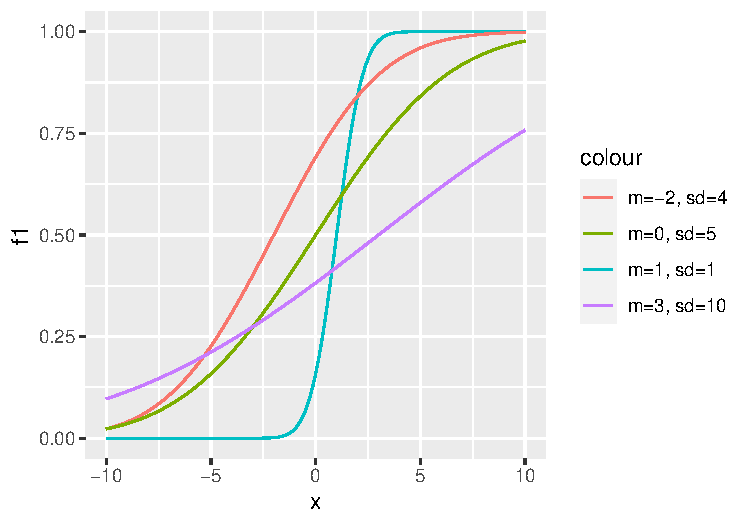
\includegraphics[width=\maxwidth]{figure/unnamed-chunk-4-1} 
\end{knitrout}
\caption{Gaussian CDF with various sets of parameters}
\label{plot2} %we can now reference plot1
\end{center}
\end{figure} 
	%%%%%%%%%%%%%%%%%%%%%%%%%%%%%%%%%%%%%%%%%%%%%%%%%%%%%%%%%%%%%%%%%%%%%%%%%%%%%%%%%%%%%%%%%%%
  %%%%%%%%%  Part (f)
  %%%%%%%%%%%%%%%%%%%%%%%%%%%%%%%%%%%%%%%%%%%%%%%%%%%%%%%%%%%%%%%%%%%%%%%%%%%%%%%%%%%%%%%%%%%
  \item Generate a random sample of size $n=10, 25, 100$, and $1000$ for your 
  two sets of parameter(s). In a $4 \times 2$ grid, plot a histogram of each set
  of data and superimpose the true density function at the specified parameter 
  values. Interpret the results.\\
  \textbf{Solution:}\\
  
\begin{knitrout}
\definecolor{shadecolor}{rgb}{0.969, 0.969, 0.969}\color{fgcolor}\begin{kframe}
\begin{alltt}
        \hlkwd{library}\hlstd{(patchwork)}
        \hlstd{sample.df} \hlkwb{<-} \hlkwd{data.frame}\hlstd{(}\hlkwc{x1}\hlstd{=}\hlkwd{rnorm}\hlstd{(}\hlnum{10}\hlstd{,} \hlkwc{mean}\hlstd{=}\hlnum{1}\hlstd{,} \hlkwc{sd}\hlstd{=}\hlnum{1}\hlstd{),}
                               \hlkwc{x2}\hlstd{=}\hlkwd{rnorm}\hlstd{(}\hlnum{25}\hlstd{,} \hlkwc{mean}\hlstd{=}\hlnum{1}\hlstd{,} \hlkwc{sd}\hlstd{=}\hlnum{1}\hlstd{),}
                               \hlkwc{x3}\hlstd{=}\hlkwd{rnorm}\hlstd{(}\hlnum{100}\hlstd{,} \hlkwc{mean}\hlstd{=}\hlnum{1}\hlstd{,} \hlkwc{sd}\hlstd{=}\hlnum{1}\hlstd{),}
                               \hlkwc{x4}\hlstd{=}\hlkwd{rnorm}\hlstd{(}\hlnum{1000}\hlstd{,} \hlkwc{mean}\hlstd{=}\hlnum{1}\hlstd{,} \hlkwc{sd}\hlstd{=}\hlnum{1}\hlstd{),}
                               \hlkwc{y1}\hlstd{=}\hlkwd{rnorm}\hlstd{(}\hlnum{10}\hlstd{,} \hlkwc{mean}\hlstd{=}\hlopt{-}\hlnum{2}\hlstd{,} \hlkwc{sd}\hlstd{=}\hlnum{4}\hlstd{),}
                               \hlkwc{y2}\hlstd{=}\hlkwd{rnorm}\hlstd{(}\hlnum{25}\hlstd{,} \hlkwc{mean}\hlstd{=}\hlopt{-}\hlnum{2}\hlstd{,} \hlkwc{sd}\hlstd{=}\hlnum{4}\hlstd{),}
                               \hlkwc{y3}\hlstd{=}\hlkwd{rnorm}\hlstd{(}\hlnum{100}\hlstd{,} \hlkwc{mean}\hlstd{=}\hlopt{-}\hlnum{2}\hlstd{,} \hlkwc{sd}\hlstd{=}\hlnum{4}\hlstd{),}
                               \hlkwc{y4}\hlstd{=}\hlkwd{rnorm}\hlstd{(}\hlnum{1000}\hlstd{,} \hlkwc{mean}\hlstd{=}\hlopt{-}\hlnum{2}\hlstd{,} \hlkwc{sd}\hlstd{=}\hlnum{4}\hlstd{))}

        \hlcom{#first line}
        \hlstd{x1}\hlkwb{<-}\hlkwd{ggplot}\hlstd{(sample.df,} \hlkwd{aes}\hlstd{(x1))}\hlopt{+}
          \hlkwd{geom_histogram}\hlstd{(}\hlkwd{aes}\hlstd{(}\hlkwc{y}\hlstd{=..density..),} \hlkwc{bins}\hlstd{=}\hlnum{10}\hlstd{,}
                         \hlkwc{color}\hlstd{=}\hlstr{"black"}\hlstd{)}\hlopt{+}
\hlkwd{geom_function}\hlstd{(}\hlkwc{fun}\hlstd{=dnorm,} \hlkwc{args} \hlstd{=} \hlkwd{list}\hlstd{(}\hlkwc{mean} \hlstd{=} \hlnum{1}\hlstd{,} \hlkwc{sd} \hlstd{=} \hlnum{1}\hlstd{),}
              \hlkwc{color}\hlstd{=}\hlstr{"red"}\hlstd{)}

        \hlstd{x2}\hlkwb{<-}\hlkwd{ggplot}\hlstd{(sample.df,} \hlkwd{aes}\hlstd{(x2))}\hlopt{+}
          \hlkwd{geom_histogram}\hlstd{(}\hlkwd{aes}\hlstd{(}\hlkwc{y}\hlstd{=..density..),} \hlkwc{bins}\hlstd{=}\hlnum{10}\hlstd{,}
                         \hlkwc{color}\hlstd{=}\hlstr{"black"}\hlstd{)}\hlopt{+}
\hlkwd{geom_function}\hlstd{(}\hlkwc{fun}\hlstd{=dnorm,} \hlkwc{args} \hlstd{=} \hlkwd{list}\hlstd{(}\hlkwc{mean} \hlstd{=} \hlnum{1}\hlstd{,} \hlkwc{sd} \hlstd{=} \hlnum{1}\hlstd{),}
              \hlkwc{color}\hlstd{=}\hlstr{"red"}\hlstd{)}

        \hlstd{x3}\hlkwb{<-}\hlkwd{ggplot}\hlstd{(sample.df,} \hlkwd{aes}\hlstd{(x3))}\hlopt{+}
          \hlkwd{geom_histogram}\hlstd{(}\hlkwd{aes}\hlstd{(}\hlkwc{y}\hlstd{=..density..),} \hlkwc{bins}\hlstd{=}\hlnum{10}\hlstd{,}
                         \hlkwc{color}\hlstd{=}\hlstr{"black"}\hlstd{)}\hlopt{+}
\hlkwd{geom_function}\hlstd{(}\hlkwc{fun}\hlstd{=dnorm,} \hlkwc{args} \hlstd{=} \hlkwd{list}\hlstd{(}\hlkwc{mean} \hlstd{=} \hlnum{1}\hlstd{,} \hlkwc{sd} \hlstd{=} \hlnum{1}\hlstd{),}
              \hlkwc{color}\hlstd{=}\hlstr{"red"}\hlstd{)}

        \hlstd{x4}\hlkwb{<-}\hlkwd{ggplot}\hlstd{(sample.df,} \hlkwd{aes}\hlstd{(x4))}\hlopt{+}
          \hlkwd{geom_histogram}\hlstd{(}\hlkwd{aes}\hlstd{(}\hlkwc{y}\hlstd{=..density..),} \hlkwc{bins}\hlstd{=}\hlnum{10}\hlstd{,}
                         \hlkwc{color}\hlstd{=}\hlstr{"black"}\hlstd{)}\hlopt{+}
\hlkwd{geom_function}\hlstd{(}\hlkwc{fun}\hlstd{=dnorm,} \hlkwc{args} \hlstd{=} \hlkwd{list}\hlstd{(}\hlkwc{mean} \hlstd{=} \hlnum{1}\hlstd{,} \hlkwc{sd} \hlstd{=} \hlnum{1}\hlstd{),}
              \hlkwc{color}\hlstd{=}\hlstr{"red"}\hlstd{)}


        \hlcom{#second line}
        \hlstd{y1}\hlkwb{<-}\hlkwd{ggplot}\hlstd{(sample.df,} \hlkwd{aes}\hlstd{(y1))}\hlopt{+}
          \hlkwd{geom_histogram}\hlstd{(}\hlkwd{aes}\hlstd{(}\hlkwc{y}\hlstd{=..density..),} \hlkwc{bins}\hlstd{=}\hlnum{10}\hlstd{,}
                         \hlkwc{color}\hlstd{=}\hlstr{"black"}\hlstd{)}\hlopt{+}
\hlkwd{geom_function}\hlstd{(}\hlkwc{fun}\hlstd{=dnorm,} \hlkwc{args} \hlstd{=} \hlkwd{list}\hlstd{(}\hlkwc{mean} \hlstd{=} \hlopt{-}\hlnum{2}\hlstd{,} \hlkwc{sd} \hlstd{=} \hlnum{4}\hlstd{),}
              \hlkwc{color}\hlstd{=}\hlstr{"red"}\hlstd{)}

        \hlstd{y2}\hlkwb{<-}\hlkwd{ggplot}\hlstd{(sample.df,} \hlkwd{aes}\hlstd{(y2))}\hlopt{+}
          \hlkwd{geom_histogram}\hlstd{(}\hlkwd{aes}\hlstd{(}\hlkwc{y}\hlstd{=..density..),} \hlkwc{bins}\hlstd{=}\hlnum{10}\hlstd{,}
                         \hlkwc{color}\hlstd{=}\hlstr{"black"}\hlstd{)}\hlopt{+}
\hlkwd{geom_function}\hlstd{(}\hlkwc{fun}\hlstd{=dnorm,} \hlkwc{args} \hlstd{=} \hlkwd{list}\hlstd{(}\hlkwc{mean} \hlstd{=} \hlopt{-}\hlnum{2}\hlstd{,} \hlkwc{sd} \hlstd{=} \hlnum{4}\hlstd{),}
              \hlkwc{color}\hlstd{=}\hlstr{"red"}\hlstd{)}

        \hlstd{y3}\hlkwb{<-}\hlkwd{ggplot}\hlstd{(sample.df,} \hlkwd{aes}\hlstd{(y3))}\hlopt{+}
          \hlkwd{geom_histogram}\hlstd{(}\hlkwd{aes}\hlstd{(}\hlkwc{y}\hlstd{=..density..),} \hlkwc{bins}\hlstd{=}\hlnum{10}\hlstd{,}
                         \hlkwc{color}\hlstd{=}\hlstr{"black"}\hlstd{)}\hlopt{+}
\hlkwd{geom_function}\hlstd{(}\hlkwc{fun}\hlstd{=dnorm,} \hlkwc{args} \hlstd{=} \hlkwd{list}\hlstd{(}\hlkwc{mean} \hlstd{=} \hlopt{-}\hlnum{2}\hlstd{,} \hlkwc{sd} \hlstd{=} \hlnum{4}\hlstd{),}
              \hlkwc{color}\hlstd{=}\hlstr{"red"}\hlstd{)}

        \hlstd{y4}\hlkwb{<-}\hlkwd{ggplot}\hlstd{(sample.df,} \hlkwd{aes}\hlstd{(y4))}\hlopt{+}
          \hlkwd{geom_histogram}\hlstd{(}\hlkwd{aes}\hlstd{(}\hlkwc{y}\hlstd{=..density..),} \hlkwc{bins}\hlstd{=}\hlnum{10}\hlstd{,}
                         \hlkwc{color}\hlstd{=}\hlstr{"black"}\hlstd{)}\hlopt{+}
\hlkwd{geom_function}\hlstd{(}\hlkwc{fun}\hlstd{=dnorm,} \hlkwc{args} \hlstd{=} \hlkwd{list}\hlstd{(}\hlkwc{mean} \hlstd{=} \hlopt{-}\hlnum{2}\hlstd{,} \hlkwc{sd} \hlstd{=} \hlnum{4}\hlstd{),}
              \hlkwc{color}\hlstd{=}\hlstr{"red"}\hlstd{)}


        \hlstd{(x1}\hlopt{|}\hlstd{x2}\hlopt{|}\hlstd{x3}\hlopt{|}\hlstd{x4)}\hlopt{/}\hlstd{(y1}\hlopt{|}\hlstd{y2}\hlopt{|}\hlstd{y3}\hlopt{|}\hlstd{y4)}
\end{alltt}
\end{kframe}
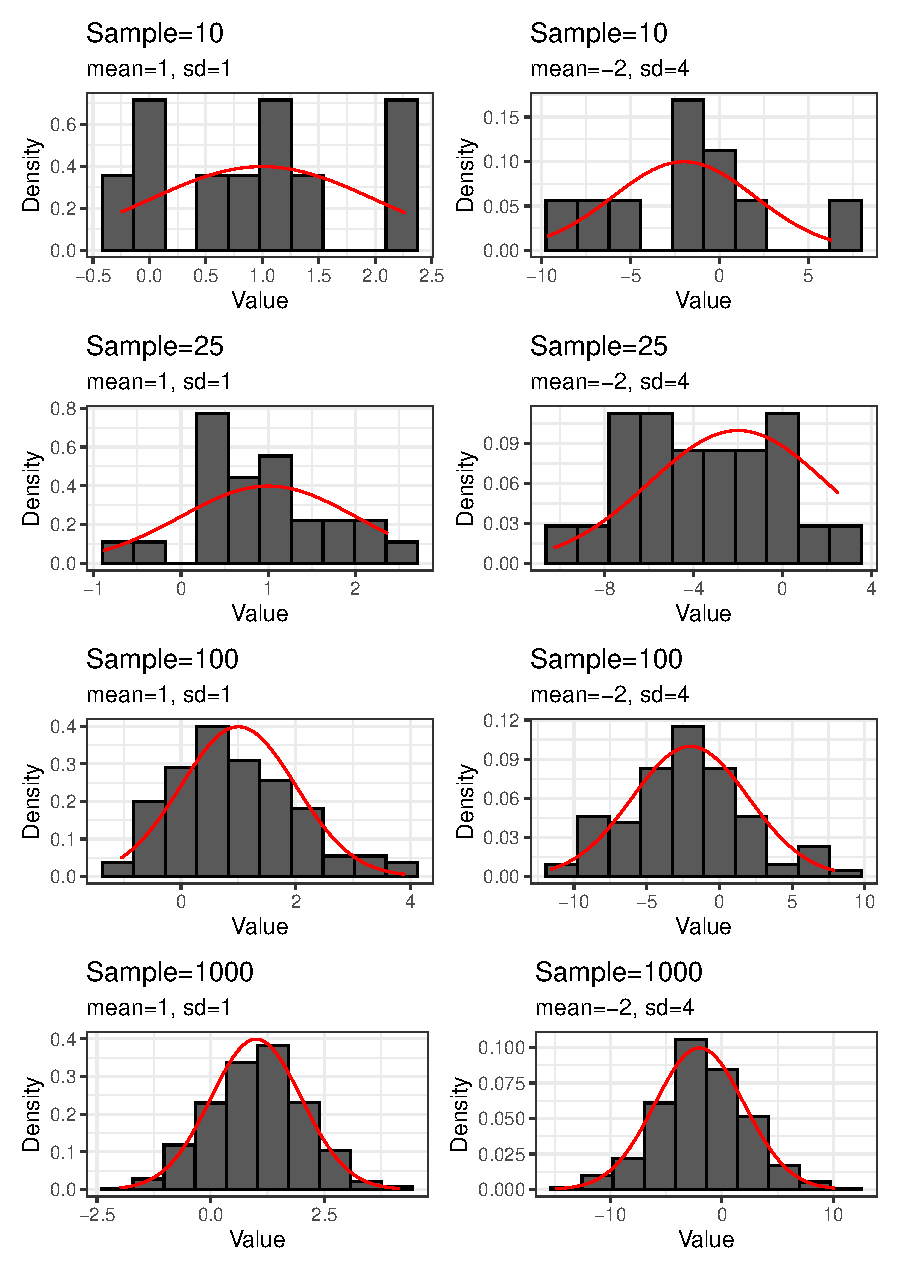
\includegraphics[width=\maxwidth]{figure/unnamed-chunk-5-1} 
\end{knitrout}
	\end{enumerate}
%%%%%%%%%%%%%%%%%%%%%%%%%%%%%%%%%%%%%%%%%%%%%%%%%%%%%%%%%%%%%%%%%%%%%%%%%%%%%%%%%%%%%%%%%%%
%%%%%%%%%%%%%%%%%%%%%%%%%%%%%%%%%%%%%%%%%%%%%%%%%%%%%%%%%%%%%%%%%%%%%%%%%%%%%%%%%%%%%%%%%%%
%%%%%%%%%  Question 2
%%%%%%%%%%%%%%%%%%%%%%%%%%%%%%%%%%%%%%%%%%%%%%%%%%%%%%%%%%%%%%%%%%%%%%%%%%%%%%%%%%%%%%%%%%%
%%%%%%%%%%%%%%%%%%%%%%%%%%%%%%%%%%%%%%%%%%%%%%%%%%%%%%%%%%%%%%%%%%%%%%%%%%%%%%%%%%%%%%%%%%%
\item Continue with the continuous distribution you selected for Question \ref{Q1}.
\begin{enumerate}
  %%%%%%%%%%%%%%%%%%%%%%%%%%%%%%%%%%%%%%%%%%%%%%%%%%%%%%%%%%%%%%%%%%%%%%%%%%%%%%%%%%%%%%%%%%%
  %%%%%%%%%  Part (a)
  %%%%%%%%%%%%%%%%%%%%%%%%%%%%%%%%%%%%%%%%%%%%%%%%%%%%%%%%%%%%%%%%%%%%%%%%%%%%%%%%%%%%%%%%%%%
  \item Provide the mean, standard deviation, skewness, and kurtosis of the PDF.
  Ensure to interpret each.
  %%%%%%%%%%%%%%%%%%%%%%%%%%%%%%%%%%%%%%%%%%%%%%%%%%%%%%%%%%%%%%%%%%%%%%%%%%%%%%%%%%%%%%%%%%%
  %%%%%%%%%  Part (b)
  %%%%%%%%%%%%%%%%%%%%%%%%%%%%%%%%%%%%%%%%%%%%%%%%%%%%%%%%%%%%%%%%%%%%%%%%%%%%%%%%%%%%%%%%%%%
  \item Generate a random sample of size $n=10, 25, 100$, and $1000$ for your 
  two sets of parameter(s). Calculate the sample mean, standard deviation, 
  skewness, and kurtosis. Interpret the results.
  %%%%%%%%%%%%%%%%%%%%%%%%%%%%%%%%%%%%%%%%%%%%%%%%%%%%%%%%%%%%%%%%%%%%%%%%%%%%%%%%%%%%%%%%%%%
  %%%%%%%%%  Part (c)
  %%%%%%%%%%%%%%%%%%%%%%%%%%%%%%%%%%%%%%%%%%%%%%%%%%%%%%%%%%%%%%%%%%%%%%%%%%%%%%%%%%%%%%%%%%%
  \item Generate a random sample of size $n=10$ for your two sets of parameter(s).
  Calculate the method of moments estimator(s) and maximum likelihood estimator(s).
  In a $1 \times 2$ grid, plot a histogram of each set of data with (1) the method 
  of moments estimated distribution, (2) the maximum likelihood estimated 
  distribution, and superimpose the true distribution in both.
  %%%%%%%%%%%%%%%%%%%%%%%%%%%%%%%%%%%%%%%%%%%%%%%%%%%%%%%%%%%%%%%%%%%%%%%%%%%%%%%%%%%%%%%%%%%
  %%%%%%%%%  Part (d)
  %%%%%%%%%%%%%%%%%%%%%%%%%%%%%%%%%%%%%%%%%%%%%%%%%%%%%%%%%%%%%%%%%%%%%%%%%%%%%%%%%%%%%%%%%%%
  \item Generate a random sample of size $n=25$ for your two sets of parameter(s).
  Calculate the method of moments estimator(s) and maximum likelihood estimator(s). 
  In a $1 \times 2$ grid, plot a histogram of each set of data with (1) the method 
  of moments estimated distribution, (2) the maximum likelihood estimated distribution, 
  and superimpose the true distribution in both.
  %%%%%%%%%%%%%%%%%%%%%%%%%%%%%%%%%%%%%%%%%%%%%%%%%%%%%%%%%%%%%%%%%%%%%%%%%%%%%%%%%%%%%%%%%%%
  %%%%%%%%%  Part (e)
  %%%%%%%%%%%%%%%%%%%%%%%%%%%%%%%%%%%%%%%%%%%%%%%%%%%%%%%%%%%%%%%%%%%%%%%%%%%%%%%%%%%%%%%%%%%
  \item Generate a random sample of size $n=100$ for your two sets of parameter(s). 
  Calculate the method of moments estimator(s) and maximum likelihood estimator(s).
  In a $1 \times 2$ grid, plot a histogram of each set of data with (1) the method 
  of moments estimated distribution, (2) the maximum likelihood estimated distribution,
  and superimpose the true distribution in both.
  %%%%%%%%%%%%%%%%%%%%%%%%%%%%%%%%%%%%%%%%%%%%%%%%%%%%%%%%%%%%%%%%%%%%%%%%%%%%%%%%%%%%%%%%%%%
  %%%%%%%%%  Part (f)
  %%%%%%%%%%%%%%%%%%%%%%%%%%%%%%%%%%%%%%%%%%%%%%%%%%%%%%%%%%%%%%%%%%%%%%%%%%%%%%%%%%%%%%%%%%%
  \item Generate a random sample of size $n=100$ for your two sets of parameter(s). 
  Calculate the method of moments estimator(s) and maximum likelihood estimator(s). 
  In a $1 \times 2$ grid, plot a histogram of each set of data with (1) the method 
  of moments estimated distribution, (2) the maximum likelihood estimated distribution, 
  and superimpose the true distribution in both.
  %%%%%%%%%%%%%%%%%%%%%%%%%%%%%%%%%%%%%%%%%%%%%%%%%%%%%%%%%%%%%%%%%%%%%%%%%%%%%%%%%%%%%%%%%%%
  %%%%%%%%%  Part (g)
  %%%%%%%%%%%%%%%%%%%%%%%%%%%%%%%%%%%%%%%%%%%%%%%%%%%%%%%%%%%%%%%%%%%%%%%%%%%%%%%%%%%%%%%%%%%
  \item Comment on the results of parts (c)-(f). 
\end{enumerate}
\newpage
%%%%%%%%%%%%%%%%%%%%%%%%%%%%%%%%%%%%%%%%%%%%%%%%%%%%%%%%%%%%%%%%%%%%%%%%%%%%%%%%%%%%%%%%%%%
%%%%%%%%%%%%%%%%%%%%%%%%%%%%%%%%%%%%%%%%%%%%%%%%%%%%%%%%%%%%%%%%%%%%%%%%%%%%%%%%%%%%%%%%%%%
%%%%%%%%%  Question 3
%%%%%%%%%%%%%%%%%%%%%%%%%%%%%%%%%%%%%%%%%%%%%%%%%%%%%%%%%%%%%%%%%%%%%%%%%%%%%%%%%%%%%%%%%%%
%%%%%%%%%%%%%%%%%%%%%%%%%%%%%%%%%%%%%%%%%%%%%%%%%%%%%%%%%%%%%%%%%%%%%%%%%%%%%%%%%%%%%%%%%%%
  \item\label{Q3} Select a discrete distribution (not the Poisson). It does not 
  have to be one that we cover in the notes! To explore the PMF of your distribution, 
  specify two sets of parameter(s) for your distribution.
  \begin{enumerate}
  %%%%%%%%%%%%%%%%%%%%%%%%%%%%%%%%%%%%%%%%%%%%%%%%%%%%%%%%%%%%%%%%%%%%%%%%%%%%%%%%%%%%%%%%%%%
  %%%%%%%%%  Part (a)
  %%%%%%%%%%%%%%%%%%%%%%%%%%%%%%%%%%%%%%%%%%%%%%%%%%%%%%%%%%%%%%%%%%%%%%%%%%%%%%%%%%%%%%%%%%%
  \item \textbf{History} Discuss what types of random variables are modeled with 
  your distribution. Be sure to include a discussion about the support and ensure
  to provide the mass function, and CDF. This requires some internet research -- 
  what's the history of the distribution, why was it created and named? What are
  some exciting applications of this distribution? Cite all of your sources.
  %%%%%%%%%%%%%%%%%%%%%%%%%%%%%%%%%%%%%%%%%%%%%%%%%%%%%%%%%%%%%%%%%%%%%%%%%%%%%%%%%%%%%%%%%%%
  %%%%%%%%%  Part (b)
  %%%%%%%%%%%%%%%%%%%%%%%%%%%%%%%%%%%%%%%%%%%%%%%%%%%%%%%%%%%%%%%%%%%%%%%%%%%%%%%%%%%%%%%%%%%
	\item Show that you have a valid PMF. You can show this approximately by 
	calculating the series in a repeat loop until probability mass evaluations are 
	infinitesimally small.
	%%%%%%%%%%%%%%%%%%%%%%%%%%%%%%%%%%%%%%%%%%%%%%%%%%%%%%%%%%%%%%%%%%%%%%%%%%%%%%%%%%%%%%%%%%%
  %%%%%%%%%  Part (c)
  %%%%%%%%%%%%%%%%%%%%%%%%%%%%%%%%%%%%%%%%%%%%%%%%%%%%%%%%%%%%%%%%%%%%%%%%%%%%%%%%%%%%%%%%%%%
	\item Find the median for your two sets of parameter(s). Conduct some research 
	to find the median based on our PMF to confirm that your numerical approach is
	correct. 
	%%%%%%%%%%%%%%%%%%%%%%%%%%%%%%%%%%%%%%%%%%%%%%%%%%%%%%%%%%%%%%%%%%%%%%%%%%%%%%%%%%%%%%%%%%%
  %%%%%%%%%  Part (d)
  %%%%%%%%%%%%%%%%%%%%%%%%%%%%%%%%%%%%%%%%%%%%%%%%%%%%%%%%%%%%%%%%%%%%%%%%%%%%%%%%%%%%%%%%%%%
	\item \label{q3PMF} Graph the PMF for several values of the parameter(s) 
	including the two sets you specified. What does changing the parameter(s) do 
	to the shape of the PMF?
	%%%%%%%%%%%%%%%%%%%%%%%%%%%%%%%%%%%%%%%%%%%%%%%%%%%%%%%%%%%%%%%%%%%%%%%%%%%%%%%%%%%%%%%%%%%
  %%%%%%%%%  Part (e)
  %%%%%%%%%%%%%%%%%%%%%%%%%%%%%%%%%%%%%%%%%%%%%%%%%%%%%%%%%%%%%%%%%%%%%%%%%%%%%%%%%%%%%%%%%%%
	 \item Graph the CDF for the same values of the parameter(s) as you did in 
	 Question \ref{q3PMF}. What does changing the parameter(s) do to the shape of 
	 the CDF? Comment on the aspects of the CDFs that show that the CDF is valid.
	%%%%%%%%%%%%%%%%%%%%%%%%%%%%%%%%%%%%%%%%%%%%%%%%%%%%%%%%%%%%%%%%%%%%%%%%%%%%%%%%%%%%%%%%%%%
  %%%%%%%%%  Part (f)
  %%%%%%%%%%%%%%%%%%%%%%%%%%%%%%%%%%%%%%%%%%%%%%%%%%%%%%%%%%%%%%%%%%%%%%%%%%%%%%%%%%%%%%%%%%%
  \item Generate a random sample of size $n=10, 25, 100$, and $1000$ for your 
  two sets of parameter(s). In a $4 \times 2$ grid, plot a histogram (with bin 
  size 1) of each set of data and superimpose the true mass function at the 
  specified parameter values. Interpret the results.
	\end{enumerate}
%%%%%%%%%%%%%%%%%%%%%%%%%%%%%%%%%%%%%%%%%%%%%%%%%%%%%%%%%%%%%%%%%%%%%%%%%%%%%%%%%%%%%%%%%%%
%%%%%%%%%%%%%%%%%%%%%%%%%%%%%%%%%%%%%%%%%%%%%%%%%%%%%%%%%%%%%%%%%%%%%%%%%%%%%%%%%%%%%%%%%%%
%%%%%%%%%  Question 2
%%%%%%%%%%%%%%%%%%%%%%%%%%%%%%%%%%%%%%%%%%%%%%%%%%%%%%%%%%%%%%%%%%%%%%%%%%%%%%%%%%%%%%%%%%%
%%%%%%%%%%%%%%%%%%%%%%%%%%%%%%%%%%%%%%%%%%%%%%%%%%%%%%%%%%%%%%%%%%%%%%%%%%%%%%%%%%%%%%%%%%%
\item Continue with the discrete distribution you selected for Question \ref{Q3}.
\begin{enumerate}
  %%%%%%%%%%%%%%%%%%%%%%%%%%%%%%%%%%%%%%%%%%%%%%%%%%%%%%%%%%%%%%%%%%%%%%%%%%%%%%%%%%%%%%%%%%%
  %%%%%%%%%  Part (a)
  %%%%%%%%%%%%%%%%%%%%%%%%%%%%%%%%%%%%%%%%%%%%%%%%%%%%%%%%%%%%%%%%%%%%%%%%%%%%%%%%%%%%%%%%%%%
  \item Provide the mean, standard deviation, skewness, and kurtosis of the PMF. 
  Ensure to interpret each.
  %%%%%%%%%%%%%%%%%%%%%%%%%%%%%%%%%%%%%%%%%%%%%%%%%%%%%%%%%%%%%%%%%%%%%%%%%%%%%%%%%%%%%%%%%%%
  %%%%%%%%%  Part (b)
  %%%%%%%%%%%%%%%%%%%%%%%%%%%%%%%%%%%%%%%%%%%%%%%%%%%%%%%%%%%%%%%%%%%%%%%%%%%%%%%%%%%%%%%%%%%
  \item Generate a random sample of size $n=10, 25, 100$, and $1000$ for your 
  two sets of parameter(s). Calculate the sample mean, standard deviation, 
  skewness, and kurtosis. Interpret the results.
  %%%%%%%%%%%%%%%%%%%%%%%%%%%%%%%%%%%%%%%%%%%%%%%%%%%%%%%%%%%%%%%%%%%%%%%%%%%%%%%%%%%%%%%%%%%
  %%%%%%%%%  Part (c)
  %%%%%%%%%%%%%%%%%%%%%%%%%%%%%%%%%%%%%%%%%%%%%%%%%%%%%%%%%%%%%%%%%%%%%%%%%%%%%%%%%%%%%%%%%%%
  \item Generate a random sample of size $n=10$ for your two sets of parameter(s).
  Calculate the method of moments estimator(s) and maximum likelihood estimator(s).
  In a $1 \times 2$ grid, plot a histogram (with bin size 1) of each set of data 
  with (1) the method of moments estimated distribution, (2) the maximum likelihood 
  estimated distribution, and superimpose the true distribution in both.
  %%%%%%%%%%%%%%%%%%%%%%%%%%%%%%%%%%%%%%%%%%%%%%%%%%%%%%%%%%%%%%%%%%%%%%%%%%%%%%%%%%%%%%%%%%%
  %%%%%%%%%  Part (d)
  %%%%%%%%%%%%%%%%%%%%%%%%%%%%%%%%%%%%%%%%%%%%%%%%%%%%%%%%%%%%%%%%%%%%%%%%%%%%%%%%%%%%%%%%%%%
  \item Generate a random sample of size $n=25$ for your two sets of parameter(s). 
  Calculate the method of moments estimator(s) and maximum likelihood estimator(s).
  In a $1 \times 2$ grid, plot a histogram (with bin size 1) of each set of data 
  with (1) the method of moments estimated distribution, (2) the maximum likelihood 
  estimated distribution, and superimpose the true distribution in both.
  %%%%%%%%%%%%%%%%%%%%%%%%%%%%%%%%%%%%%%%%%%%%%%%%%%%%%%%%%%%%%%%%%%%%%%%%%%%%%%%%%%%%%%%%%%%
  %%%%%%%%%  Part (e)
  %%%%%%%%%%%%%%%%%%%%%%%%%%%%%%%%%%%%%%%%%%%%%%%%%%%%%%%%%%%%%%%%%%%%%%%%%%%%%%%%%%%%%%%%%%%
  \item Generate a random sample of size $n=100$ for your two sets of parameter(s).
  Calculate the method of moments estimator(s) and maximum likelihood estimator(s). 
  In a $1 \times 2$ grid, plot a histogram (with bin size 1) of each set of data 
  with (1) the method of moments estimated distribution, (2) the maximum likelihood
  estimated distribution, and superimpose the true distribution in both.
  %%%%%%%%%%%%%%%%%%%%%%%%%%%%%%%%%%%%%%%%%%%%%%%%%%%%%%%%%%%%%%%%%%%%%%%%%%%%%%%%%%%%%%%%%%%
  %%%%%%%%%  Part (f)
  %%%%%%%%%%%%%%%%%%%%%%%%%%%%%%%%%%%%%%%%%%%%%%%%%%%%%%%%%%%%%%%%%%%%%%%%%%%%%%%%%%%%%%%%%%%
  \item Generate a random sample of size $n=100$ for your two sets of parameter(s).
  Calculate the method of moments estimator(s) and maximum likelihood estimator(s).
  In a $1 \times 2$ grid, plot a histogram (with bin size 1) of each set of data 
  with (1) the method of moments estimated distribution, (2) the maximum likelihood
  estimated distribution, and superimpose the true distribution in both.
  %%%%%%%%%%%%%%%%%%%%%%%%%%%%%%%%%%%%%%%%%%%%%%%%%%%%%%%%%%%%%%%%%%%%%%%%%%%%%%%%%%%%%%%%%%%
  %%%%%%%%%  Part (g)
  %%%%%%%%%%%%%%%%%%%%%%%%%%%%%%%%%%%%%%%%%%%%%%%%%%%%%%%%%%%%%%%%%%%%%%%%%%%%%%%%%%%%%%%%%%%
  \item Comment on the results of parts (c)-(f). 
\end{enumerate}
\end{enumerate}%End overall enumerate
\newpage
\bibliography{bib}
\end{document}
